\documentclass[10pt,letterpaper]{article}
% Compile with xelatex twice (or latexmk -xelatex). Figures are in figures/.
\usepackage[letterpaper,left=0.77in,right=0.77in,top=0.83in,bottom=0.77in,headheight=21pt,headsep=0.15in,footskip=0.38in]{geometry}
\usepackage{fontspec}
\IfFontExistsTF{Carlito}{\setmainfont{Carlito}}{\setmainfont{TeX Gyre Heros}}
\IfFontExistsTF{Carlito}{\setsansfont{Carlito}}{\setsansfont{TeX Gyre Heros}}
\usepackage{unicode-math}
\setmathfont{Latin Modern Math}
\usepackage[table]{xcolor}
\definecolor{navy}{HTML}{233650}
\definecolor{teal}{HTML}{277970}
\definecolor{muted}{HTML}{5A6C7D}
\definecolor{pale}{HTML}{F1F5F8}
\definecolor{textink}{HTML}{2A3440}
\usepackage{graphicx,booktabs,longtable,array,calc,ragged2e}
\usepackage{microtype}
\usepackage{float,caption,subcaption,needspace}
\usepackage{titlesec,fancyhdr}
\usepackage[hidelinks]{hyperref}
\setlength{\parindent}{0pt}
\setlength{\parskip}{5pt}
\renewcommand{\baselinestretch}{1.09}
\color{textink}
\setcounter{secnumdepth}{0}
\titleformat{\section}{\large\bfseries\color{navy}}{}{0pt}{}
\titleformat{\subsection}{\normalsize\bfseries\color{navy}}{}{0pt}{}
\titlespacing*{\section}{0pt}{11pt}{5pt}
\titlespacing*{\subsection}{0pt}{9pt}{4pt}
\captionsetup{font=footnotesize,labelfont=bf,textfont=it,justification=centering}
% Top and bottom horizontal rules: fancyhdr headrule and footrule.
\pagestyle{fancy}
\fancyhf{}
\fancyhead[R]{\textcolor{teal}{\footnotesize\bfseries DATA 37711 / HOMEWORK 2}}
\fancyfoot[C]{\textcolor{muted}{\footnotesize Homework 2 $\boldsymbol{\cdot}$ Analysis and submission\quad $\vert$\quad \thepage}}
\renewcommand{\headrulewidth}{0.45pt}
\renewcommand{\footrulewidth}{0.45pt}
\renewcommand{\headrule}{\hbox to\headwidth{\color{teal}\leaders\hrule height \headrulewidth\hfill}}
\renewcommand{\footrule}{\hbox to\headwidth{\color{teal}\leaders\hrule height \footrulewidth\hfill}}
\begin{document}
{\fontsize{21}{23}\selectfont\bfseries\color{navy} HOMEWORK 2}\par
{\small\color{muted} DATA 37711 $\cdot$ Foundations of Machine Learning \& AI $\cdot$ Autumn 2026}\par
\vspace{3pt}
\textbf{Elina Lee \textbar{} Problems 1--3}

Three experiments: uncertainty-aware taxi prediction, high-cardinality
retail prediction, and random-feature regression versus a
one-hidden-layer neural network.

\section{Summary of results}\label{summary-of-results}

\begin{center}
\begingroup
\small
\setlength{\tabcolsep}{4pt}
\renewcommand{\arraystretch}{1.18}
\rowcolors{2}{pale}{white}
\begin{tabular}{>{\raggedright\arraybackslash}p{0.290\linewidth}>{\raggedright\arraybackslash}p{0.590\linewidth}}
\rowcolor{navy}
\textcolor{white}{\textbf{Component}} & \textcolor{white}{\textbf{Selection and observed outcome}} \\
Problem 1: conditional Normal & Taxi MLP, early-stopped at the best validation epoch (169): test Brier 0.003343 vs baseline 0.004495; accuracy 99.6065\% vs 99.5505\%. \\
Problem 2: retail & Embedding-only MLP has the smallest test log-MSE (0.281836), versus hybrid 0.283321 and ridge 0.409972. \\
Problem 3: RKS / MLP & RKS D=20: validation MSE 0.036124; MLP 128 hidden units: 0.038674. Both are close to the RBF kernel-ridge limit (0.0359); the gap is within validation error. The 200-row test split is unlabeled. \\
\end{tabular}
\endgroup
\end{center}

All reported numbers come from the code in the \path{homework_2/}
directory of the course repository and can be regenerated with
\texttt{python run\_all.py -{}-problem all}. Figures 5--9 are written by
the Problem 3 scripts and Figures 1--4 by \path{code/report_figures.py}
from the data and the Problem 2 result tables (Figure 1 is an
illustrative sketch, not data). Ridge and RKS
results are deterministic; MLP results can move in the fourth decimal
place across PyTorch versions and hardware.

\section{1. Conditional mean, uncertainty, and taxi
duration}\label{conditional-mean-uncertainty-and-taxi-duration}

\subsection{1(a) Link functions}\label{a-link-functions}

The neural network produces two unconstrained real numbers, g₁(x) and
g₂(x). We use the first directly as the conditional mean, while
transforming the second through softplus plus a small positive constant
to obtain a valid conditional standard deviation. Unlike exp, softplus
grows approximately linearly for large positive values while remaining
positive.

\[\mu(x)=g_1(x),\qquad \sigma(x)=\log(1+e^{g_2(x)})+10^{-3}\]

The mean may be any real number, but the conditional standard deviation
must be strictly positive. The Normal model is the assumption requested
in the assignment, not a claim that real taxi times are exactly
Gaussian.

\subsection{1(b) Training loss from the Normal
likelihood}\label{b-training-loss-from-the-normal-likelihood}

For observation i, assume Yᵢ conditional on Xᵢ follows Normal(μᵢ, σᵢ²).
Taking minus the logarithm of the Normal density yields the per-example
negative log-likelihood. The constant term may be dropped during fitting
without changing the minimizer.

\[\ell_i=\frac{1}{2}\log(2\pi)+\log\sigma_i+\frac{(y_i-\mu_i)^2}{2\sigma_i^2}\]

The log σ term discourages arbitrarily large predicted uncertainty,
while the standardized squared-residual term discourages unrealistically
small uncertainty. Minimizing the average over the training set jointly
learns location and noise scale.

\subsection{1(c) PyTorch MLP and
baseline}\label{c-pytorch-mlp-and-baseline}

We used the supplied seven standardized trip features, with a 7→64→2
ReLU MLP, Adam (learning rate 0.002) and mini-batches of 2,048 trips. A
constant Normal baseline predicts the training-set mean and standard
deviation for every trip. The seed-42 row split comprises 366,487
training, 78,533 validation, and 78,534 test examples.

The number of epochs is chosen on the validation split: we train for at
most 300 epochs, keep the checkpoint with the lowest validation NLL, and
stop after 30 epochs without improvement. Validation NLL falls steeply
for about 130 epochs and then flattens near 2.72; the best checkpoint is
epoch 169 (validation NLL 2.7186), and training stopped at epoch 199. A
short fixed budget would not be enough here: after 12 epochs the
validation NLL is still 3.273 and falling.

\subsection{1(d) Probability of finishing in less than 45
minutes}\label{d-probability-of-finishing-in-less-than-45-minutes}

The probability is the area under each observation's fitted Normal
density to the left of the 45-minute threshold. Using the standard
Normal cumulative distribution function Φ gives:

\[p_i=P(Y_i<45\mid X_i)=\Phi\!\left(\frac{45-\mu_i}{\sigma_i}\right)\]

\begin{center}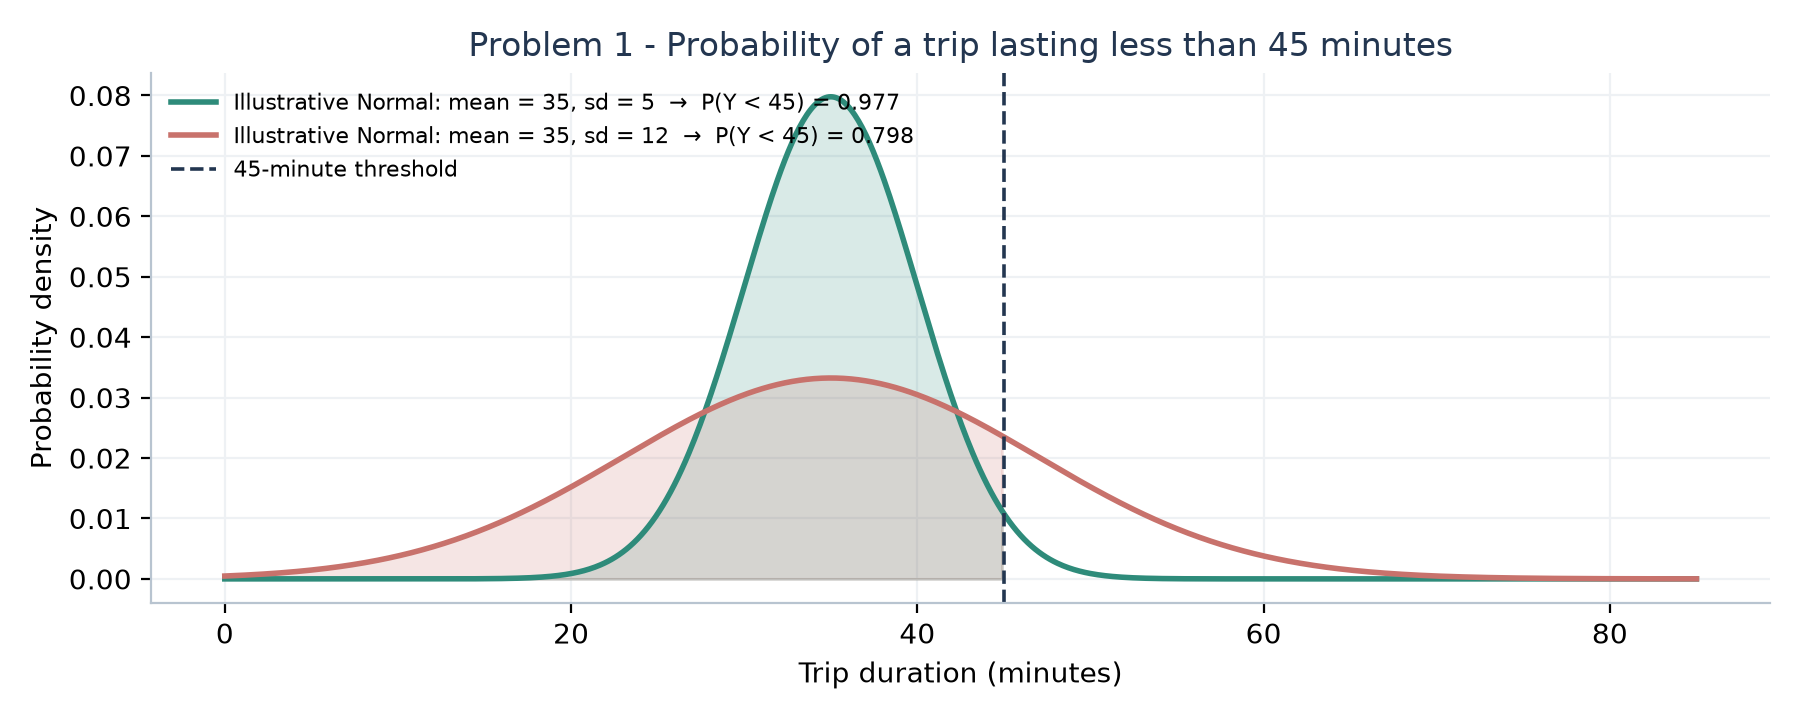
\includegraphics[width=0.88\linewidth]{figures/P1_gaussian_probability_explained.png}\end{center}

{\footnotesize\itshape\color{muted} Figure 1. Illustrative Normal densities showing why both mean and scale affect the predicted probability; not an observed-data plot.}

\subsection{1(e) Proper probability scoring and
classification}\label{e-proper-probability-scoring-and-classification}

Let zᵢ=1\{yᵢ\textless45\}. We report the Brier score, n⁻¹Σ(pᵢ−zᵢ)², a
strictly proper probability scoring rule, and classification accuracy
after thresholding pᵢ at 0.5. We additionally report Normal NLL for the
continuous response.

\begin{center}
\begingroup
\small
\setlength{\tabcolsep}{4pt}
\renewcommand{\arraystretch}{1.18}
\rowcolors{2}{pale}{white}
\begin{tabular}{>{\raggedright\arraybackslash}p{0.317\linewidth}>{\raggedright\arraybackslash}p{0.194\linewidth}>{\raggedright\arraybackslash}p{0.167\linewidth}>{\raggedright\arraybackslash}p{0.202\linewidth}}
\rowcolor{navy}
\textcolor{white}{\textbf{Model}} & \textcolor{white}{\textbf{Test NLL}} & \textcolor{white}{\textbf{Brier $\downarrow$}} & \textcolor{white}{\textbf{Accuracy}} \\
Constant Normal & 3.476824 & 0.004495 & 99.5505\% \\
Heteroscedastic MLP & 2.706100 & 0.003343 & 99.6065\% \\
\end{tabular}
\endgroup
\end{center}

The MLP improves the Brier score by about 25.6\% relative to the
constant baseline and raises accuracy from 99.5505\% to 99.6065\%. The
accuracy gain looks small because the event is so common: about 99.55\%
of trips last less than 45 minutes, so the baseline is already right
whenever it predicts ``short'' for every trip. The informative part is
the rare class. In the test split, 353 trips lasted at least 45
minutes; the baseline flags none of them, while the MLP flags 121 (34\%)
at the cost of 77 false alarms among the 78,181 shorter trips (309
errors in total versus 353). The Brier score captures this improvement
directly, which is why we report it alongside accuracy.

\clearpage
\section{2. High-cardinality retail
transactions}\label{high-cardinality-retail-transactions}

\subsection{2(a) Dataset, cardinality, and train/validation/test
split}\label{a-dataset-cardinality-and-trainvalidationtest-split}

The original retail dataset contains 397,924 transactions, with 3,665
unique StockCode values and 4,339 unique CustomerID values. Both inputs
are categorical identifiers: their numerical or lexical order does not
express a meaningful magnitude. Dense one-hot encoding for all 8,004
categories would require about 12.74 GB in float32 for the full input
matrix alone; sparse one-hot encoding is still feasible because each row
has only two nonzero features. Target encoding and embeddings are
compact alternatives.

After a seed-42 NumPy random permutation of rows, we used a common
70/15/15 split: 278,546 training, 59,689 validation, and 59,689 test
observations. All encoders and scalers use training information only. We
reserve validation for hyperparameters and early stopping, and do not
use test outcomes to select model settings. A row-level split measures
generalization to new transactions, not specifically to entirely new
customers.

Quantity is strongly heavy-tailed: median 6, 90th percentile 24, 99th
percentile 120, 99.9th percentile 504, and maximum 80,995. This
motivates a log-target loss rather than raw MSE alone.

\begin{center}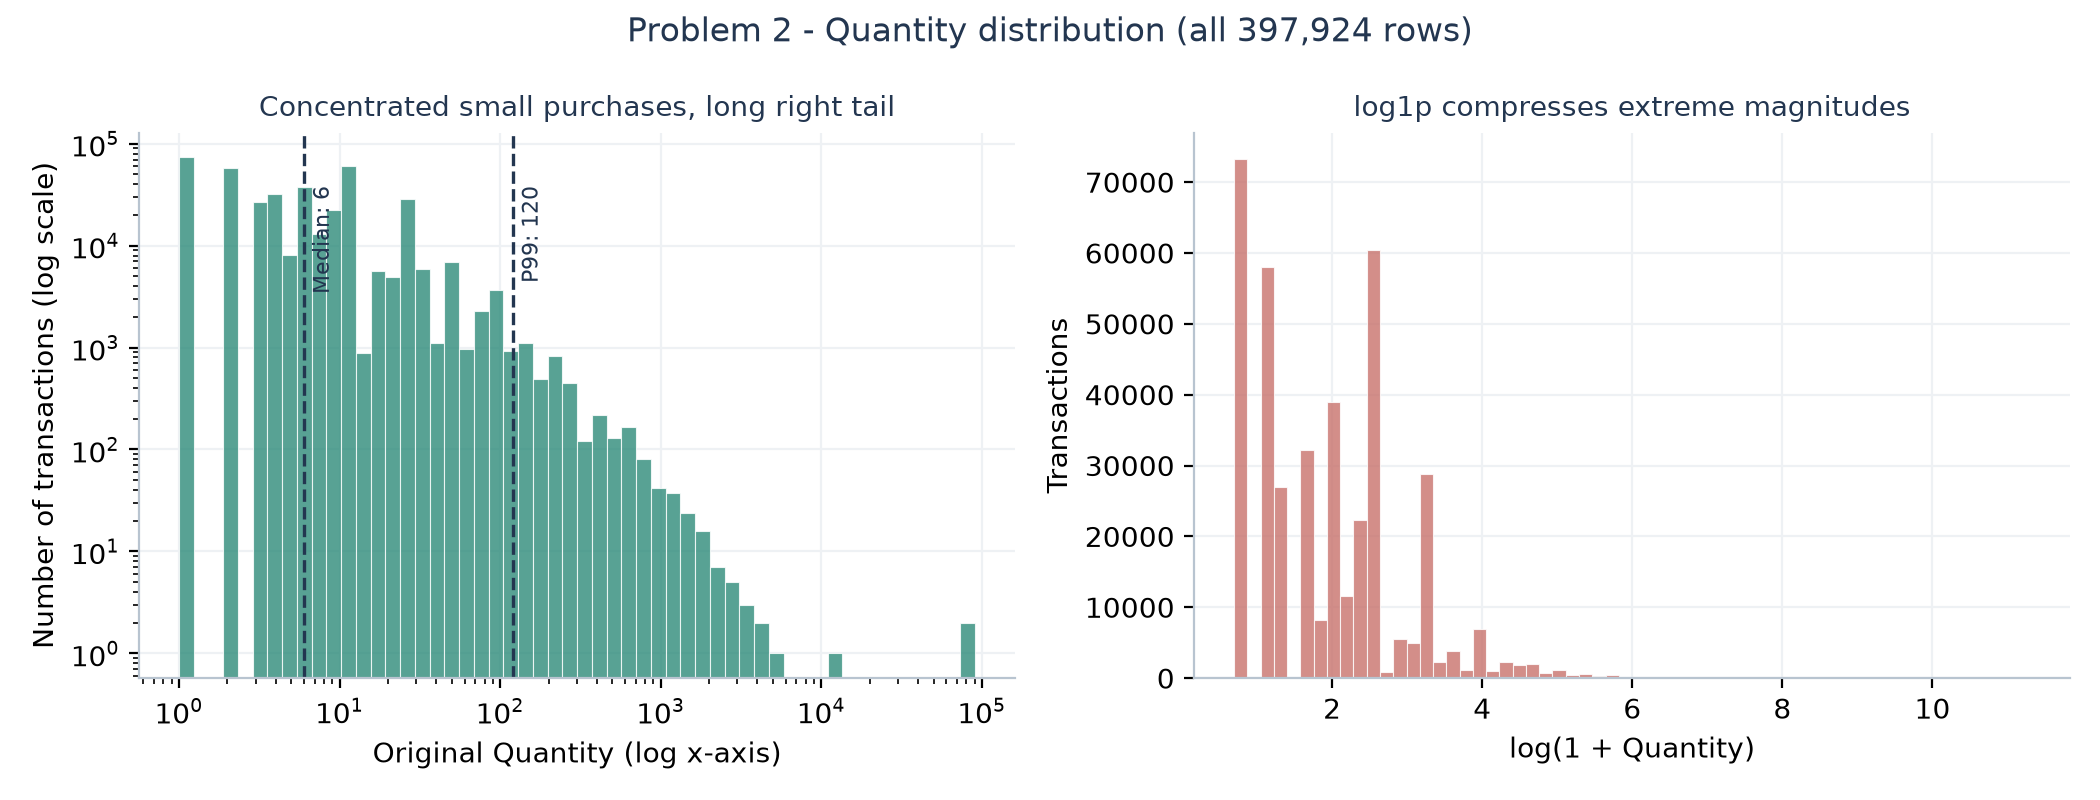
\includegraphics[width=0.91\linewidth]{figures/P2_quantity_heavy_tail.png}\end{center}

{\footnotesize\itshape\color{muted} Figure 2. Actual retail quantity distribution before and after log1p transformation, using all 397,924 supplied rows.}

\subsection{2(b) Target encoding, ridge, and validation
selection}\label{b-target-encoding-ridge-and-validation-selection}

For each product or customer category, target encoding substitutes the
mean of original Quantity calculated in a reference training subset. We
use five-fold out-of-fold encoding on the training rows so that a row
does not contribute its own target to its encoded representation.
Validation and test categories use full training-set statistics; unseen
values receive the reference training mean.

We apply log1p to both encoded predictors and response, and standardize
the encoded predictors using training means and standard deviations
only. The response transformed as t=log(1+Quantity) is then modeled
using ridge regression, leaving the intercept unpenalized.

\[\min_{\beta}\ \lVert A\beta-t\rVert_2^2+\alpha\,\beta^\top D\beta,\qquad D=\operatorname{diag}(0,1,1)\]

Differentiation yields (AᵀA+αD)β=Aᵀt. We solved the linear system with
NumPy and matched the coefficients against scikit-learn Ridge and
PyTorch, using a numerically stable solve rather than a literal inverse.
We evaluated $\alpha\in$ \{0.1, 1, 10, 100, 1000\} by validation log-MSE; α=0.1
achieved the lowest value (approximately 0.402670), with nearly
indistinguishable scores across several candidates. Although 0.1 is the
smallest value tried, a smaller α would not help: with 278,546 rows and
two standardized predictors the diagonal of AᵀA is about 2.8×10⁵, so any
α up to 10 barely moves the solution (validation log-MSE 0.402670 for
α = 0.1, 1 and 10), and α→0 is ordinary least squares.

\begin{center}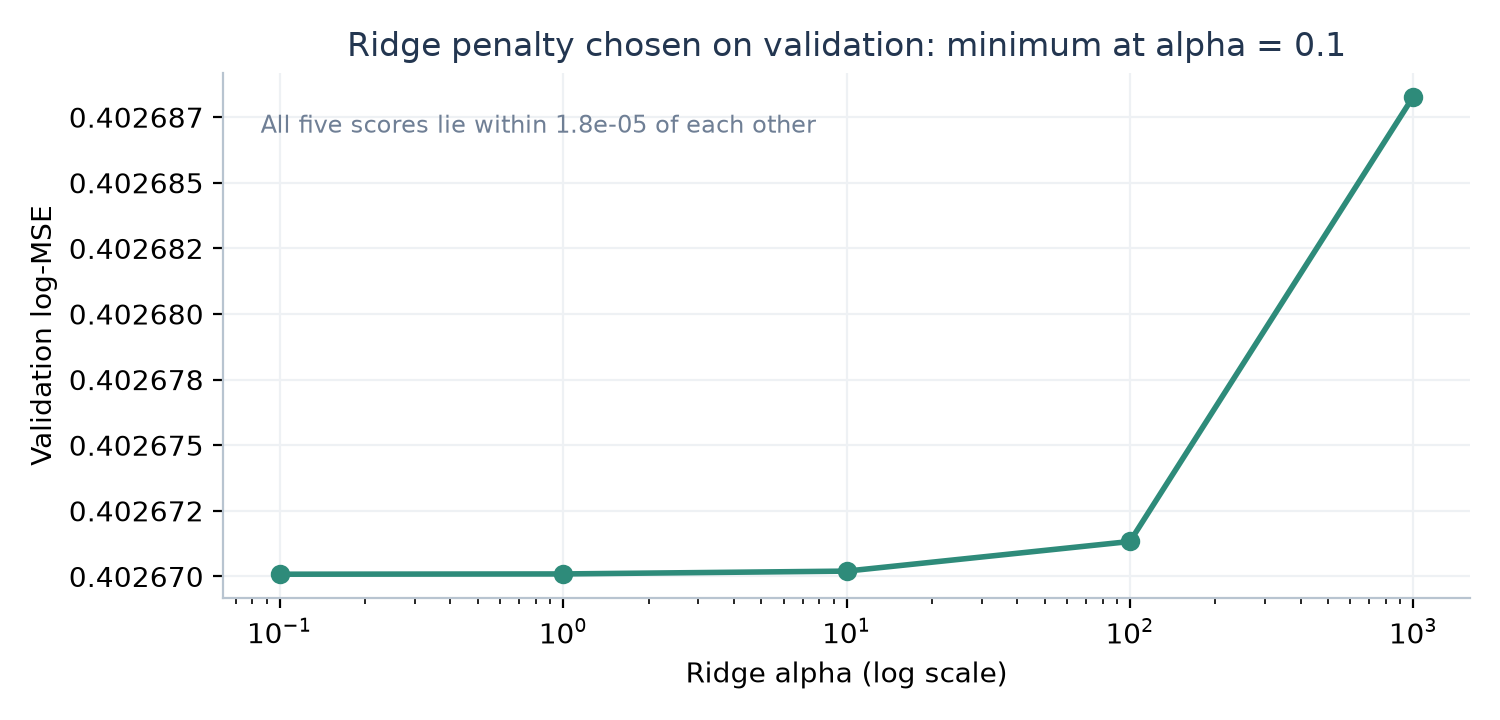
\includegraphics[width=0.73\linewidth]{figures/P2_ridge_alpha_sweep.png}\end{center}

{\footnotesize\itshape\color{muted} Figure 3. Ridge penalty selection uses validation loss only. The ordinate range is narrow; apparent changes should not be exaggerated.}

Test log-MSE for the selected ridge model was 0.409972, versus 1.009571
for the constant log-mean baseline. The ridge model also improved test
MAE from 11.6955 to 8.5201. Raw-scale RMSE decreased modestly from
307.1146 to 305.9164, consistent with the influence of extreme
transaction quantities.

\subsection{2(c) Separate categorical
embeddings}\label{c-separate-categorical-embeddings}

We trained product and customer embedding tables separately, with
embedding dimension 8 each. This follows the common rule of thumb of
roughly the fourth root of the number of categories
($3665^{1/4}\approx 7.8$ and $4339^{1/4}\approx 8.1$), and keeps the two
tables small (about 63,000 parameters) relative to 278,546 training rows. The 16 resulting features feed an MLP with
one 32-unit ReLU hidden layer and a scalar output. We used log-MSE, Adam
(learning rate 0.001), batch size 1,024, weight decay 10⁻⁵, and
validation-based early stopping (patience 10, up to 300 epochs). The
best validation loss came at epoch 98 and training stopped at epoch 108,
so the epoch budget does not bind. Unseen categories map to a reserved
index 0. The test log-MSE is 0.281836 and
MAE is 7.3757, both better than the target-encoding ridge model.

\subsection{2(d) Hybrid embeddings plus target
encodings}\label{d-hybrid-embeddings-plus-target-encodings}

The hybrid model concatenates the two 8-dimensional categorical
embeddings and the two standardized target-encoded values, yielding an
18-dimensional input to the same one-hidden-layer MLP (best epoch 61,
stopped at epoch 71). All comparison models use the same split, log
target, and evaluation metrics. Its test
log-MSE is 0.283321 and MAE 7.4918. More input information did not yield
a measurable improvement over the embedding-only model on this split.

\subsection{2(e) Test comparison and
interpretation}\label{e-test-comparison-and-interpretation}

\begin{center}
\begingroup
\small
\setlength{\tabcolsep}{4pt}
\renewcommand{\arraystretch}{1.18}
\rowcolors{2}{pale}{white}
\begin{tabular}{>{\raggedright\arraybackslash}p{0.317\linewidth}>{\raggedright\arraybackslash}p{0.141\linewidth}>{\raggedright\arraybackslash}p{0.132\linewidth}>{\raggedright\arraybackslash}p{0.123\linewidth}>{\raggedright\arraybackslash}p{0.167\linewidth}}
\rowcolor{navy}
\textcolor{white}{\textbf{Test model}} & \textcolor{white}{\textbf{Log-MSE $\downarrow$}} & \textcolor{white}{\textbf{RMSLE $\downarrow$}} & \textcolor{white}{\textbf{MAE $\downarrow$}} & \textcolor{white}{\textbf{RMSE $\downarrow$}} \\
constant baseline & 1.009571 & 1.004774 & 11.6955 & 307.1146 \\
target encoding + ridge & 0.409972 & 0.640291 & 8.5201 & 305.9164 \\
two embeddings + MLP & \textbf{0.281836} & \textbf{0.530882} & \textbf{7.3757} & \textbf{305.6237} \\
target encoding + embeddings + MLP & 0.283321 & 0.532279 & 7.4918 & 306.2395 \\
\end{tabular}
\endgroup
\end{center}

\begin{center}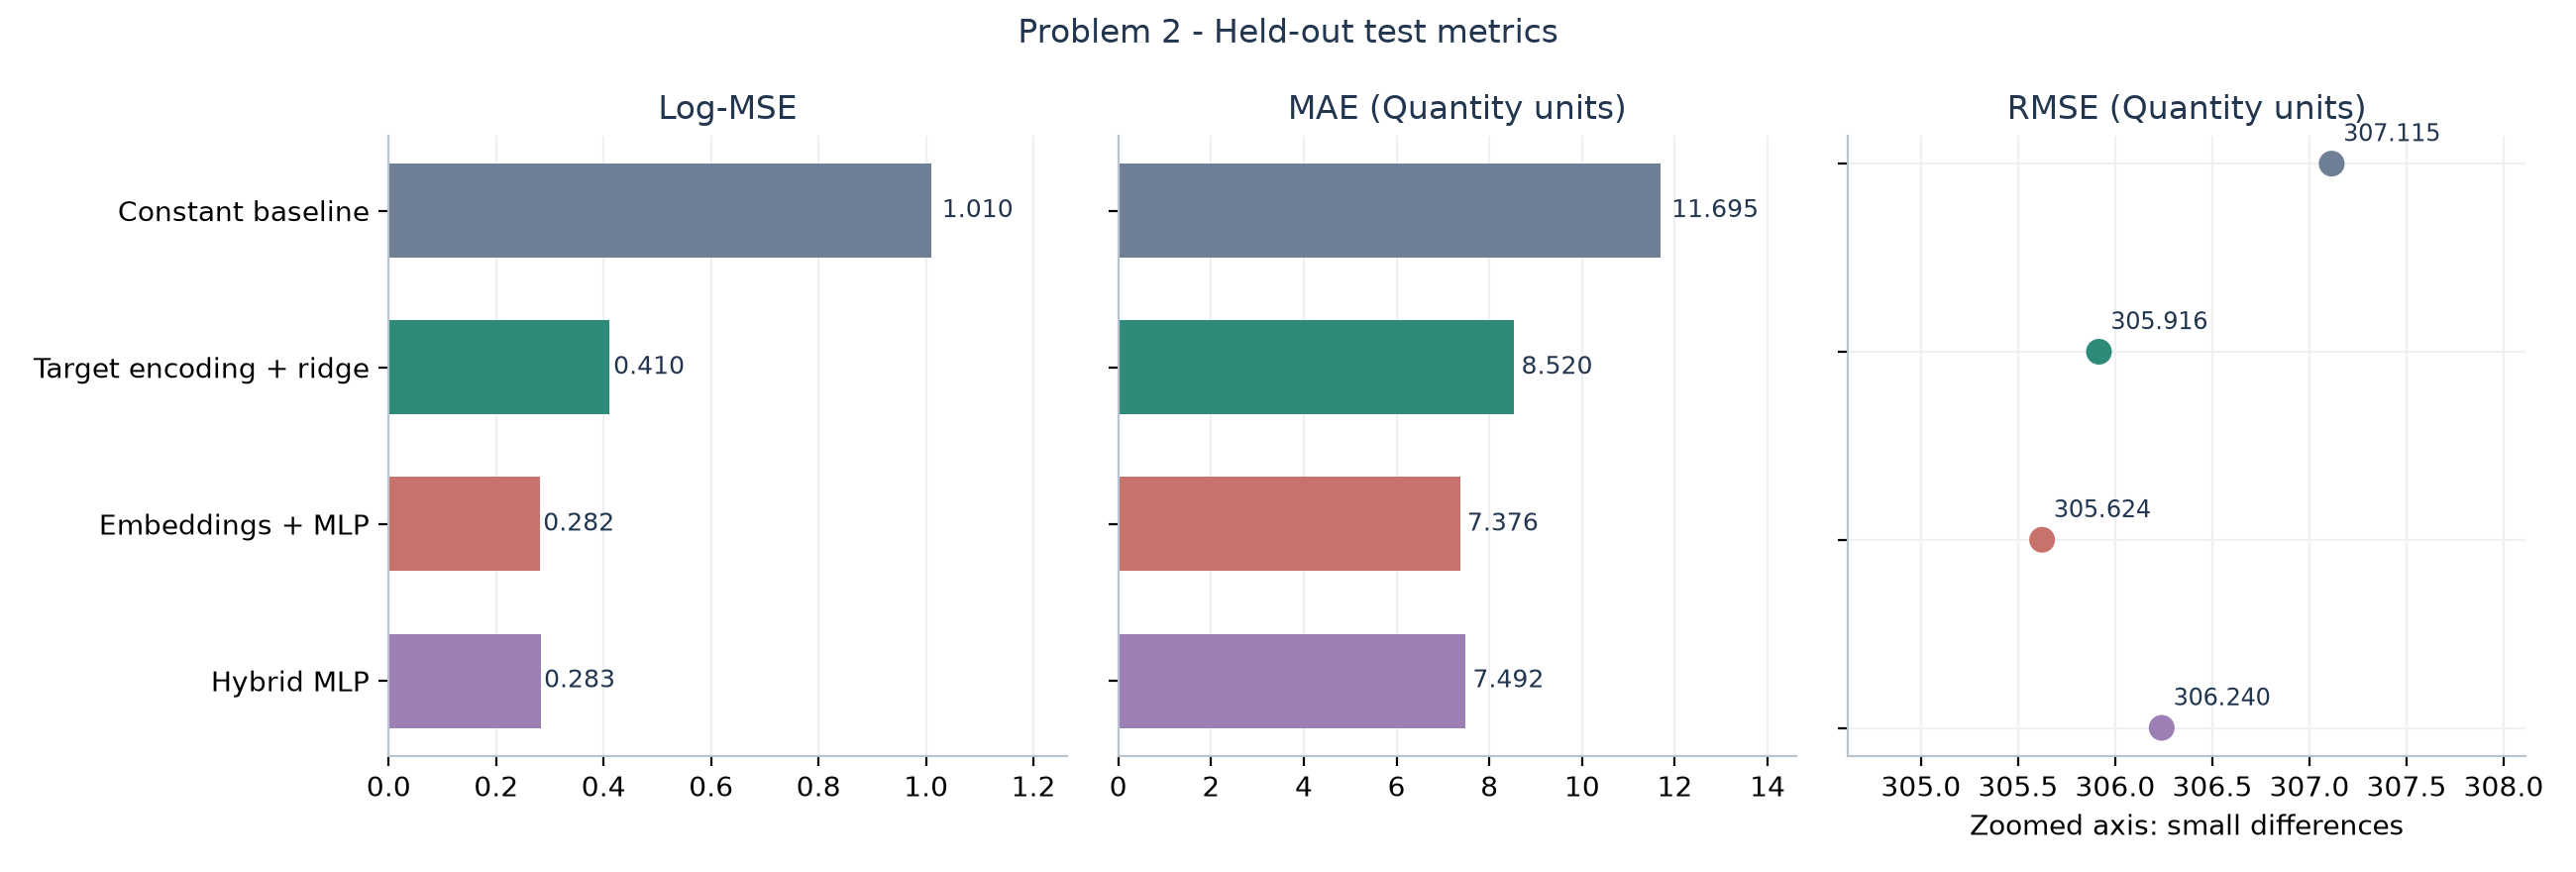
\includegraphics[width=0.90\linewidth]{figures/P2_model_metrics.png}\end{center}

{\footnotesize\itshape\color{muted} Figure 4. All four metrics on the held-out test set. RMSE uses a zoomed horizontal axis and differs only modestly between models.}

The embedding-only MLP achieved the lowest test log-MSE (0.281836),
approximately 31.3\% below the ridge model.

\textbf{What the embedding layer does.} An embedding layer is a learned
lookup table: product $i$ is mapped to row $i$ of a $3604\times 8$ weight
matrix, which is exactly a one-hot vector multiplied by that matrix,
without ever building the one-hot matrix. The rows are trained by
backpropagation together with the MLP, so products (or customers) that
behave alike end up with nearby vectors and share statistical strength,
and the hidden layer can combine the two vectors to model
product--customer interactions. Target encoding instead collapses each ID
to a single number, its mean quantity, so it cannot express that the same
product is bought in large quantities by some customers and in small
quantities by others.

\textbf{Checking this on the test set.} If the gain comes from learned
per-ID information, it should be largest for IDs seen often in training
and should disappear for IDs never seen in training, which all share the
reserved index 0. The table splits the test rows by how often their ID
appears in the training split (from the reproducibility rerun, whose
overall neural-model scores differ from the table above by at most
0.0006).

\begin{center}
\begingroup
\small
\setlength{\tabcolsep}{4pt}
\renewcommand{\arraystretch}{1.15}
\rowcolors{2}{pale}{white}
\begin{tabular}{>{\raggedright\arraybackslash}p{0.150\linewidth}>{\raggedright\arraybackslash}p{0.150\linewidth}>{\raggedright\arraybackslash}p{0.110\linewidth}>{\raggedright\arraybackslash}p{0.120\linewidth}>{\raggedright\arraybackslash}p{0.150\linewidth}>{\raggedright\arraybackslash}p{0.120\linewidth}}
\rowcolor{navy}
\textcolor{white}{\textbf{ID}} & \textcolor{white}{\textbf{Seen in train}} & \textcolor{white}{\textbf{Test rows}} & \textcolor{white}{\textbf{Ridge}} & \textcolor{white}{\textbf{Embeddings}} & \textcolor{white}{\textbf{Hybrid}} \\
StockCode & 100+ times & 42,155 & 0.399 & 0.277 & 0.277 \\
StockCode & 10--99 & 16,699 & 0.434 & 0.293 & 0.298 \\
StockCode & 1--9 & 804 & 0.476 & 0.357 & 0.345 \\
CustomerID & 100+ times & 36,042 & 0.412 & 0.296 & 0.299 \\
CustomerID & 10--99 & 22,506 & 0.386 & 0.245 & 0.247 \\
CustomerID & 1--9 & 1,118 & 0.745 & 0.448 & 0.437 \\
CustomerID & never & 23 & 4.897 & 7.450 & 4.980 \\
\end{tabular}
\endgroup
\end{center}

{\footnotesize\itshape\color{muted} Test log-MSE by training frequency of the ID (31 test rows with an unseen StockCode are omitted; too few to compare).}

The pattern matches the explanation. For well-represented IDs the
embedding model lowers log-MSE by about 0.12--0.14 relative to ridge. For
the 23 test rows from customers never seen in training it is much worse
than ridge (7.45 vs 4.90): its customer vector is the shared ``unknown''
row, which no training example updates, whereas target encoding falls back
to the training mean. The hybrid model, which also receives the
target-encoded inputs, recovers almost all of that loss (4.98) and is
slightly better for rare customers (0.437 vs 0.448). Those groups are a
very small share of the 59,689 test rows, which is why the two neural
models are tied overall; the hybrid design would matter more in a setting
with many new customers. The small overall hybrid-versus-embedding
difference should not be treated as statistically established from a
single split.

The RMSE scale needs particular care: the largest test transaction has
Quantity=74,215. For the constant baseline, this one observation
accounts for 97.8\% of total squared error. Therefore the raw-scale RMSE
is dominated by an extreme outcome and can remain close across models
even when typical log-scale and absolute errors improve. We should not
adjust architectures based on these test results; any new exploration
belongs on validation data followed by a fresh independent test.

\clearpage
\section{3. Random Kitchen Sinks versus a one-hidden-layer
MLP}\label{random-kitchen-sinks-versus-a-one-hidden-layer-mlp}

\subsection{3(a) Visualization of training
data}\label{a-visualization-of-training-data}

The supplied regression toy dataset has 600 labeled training rows, 200
labeled validation rows, and 200 unlabeled test rows, each with two
input coordinates in {[}−3,3{]}. We visualize (x₁,x₂) positions and
encode observed y with color. The training pattern is distinctly
nonlinear: values are low around the left-center and rise toward the top
and bottom, with a nonuniform horizontal trend.

\begin{center}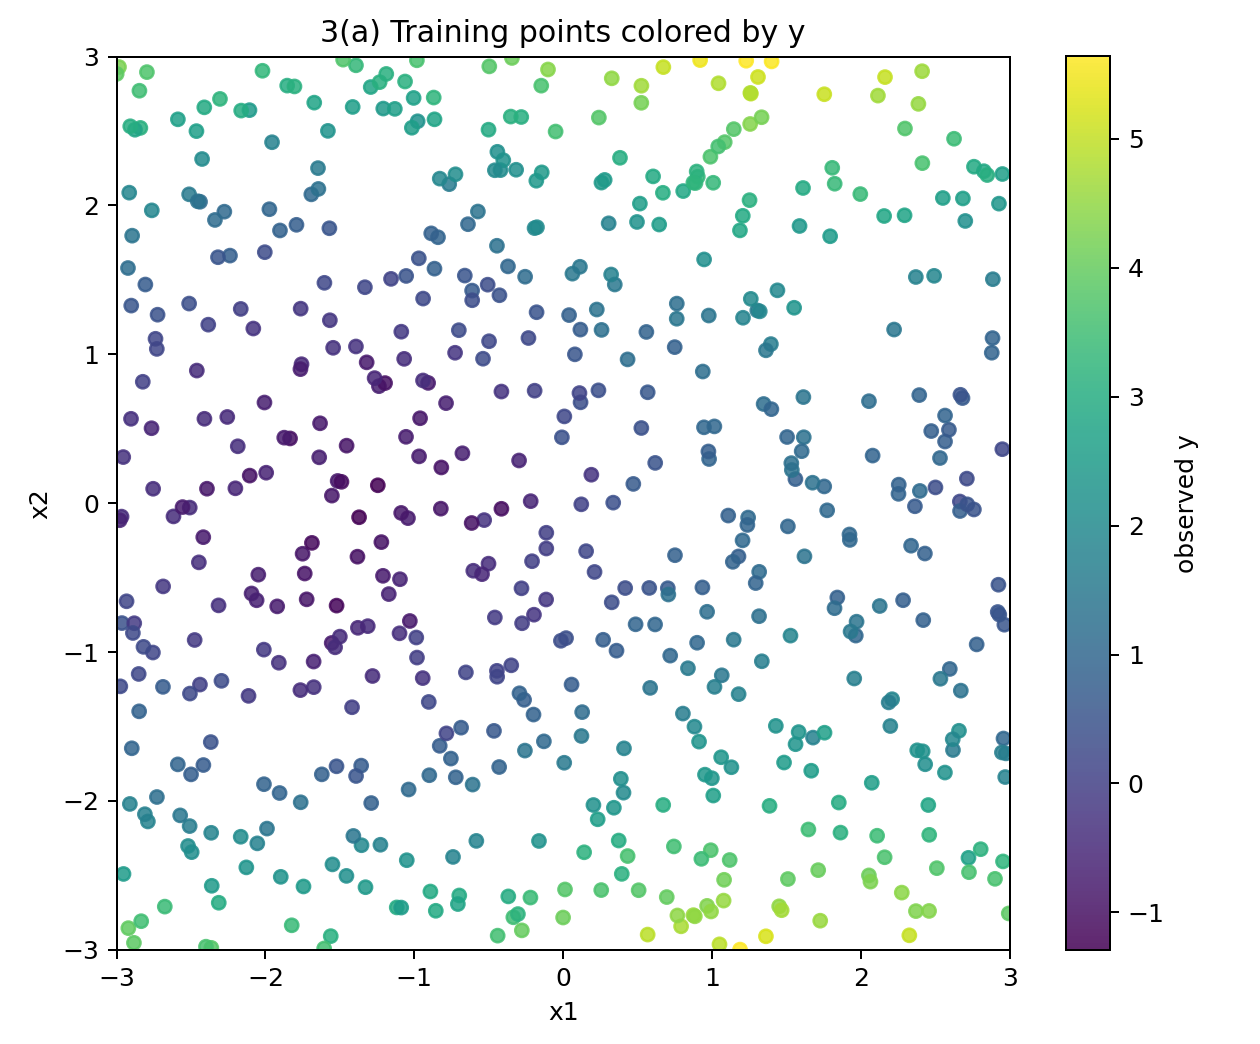
\includegraphics[width=0.65\linewidth]{figures/3a_training_scatter.png}\end{center}

{\footnotesize\itshape\color{muted} Figure 5. Original labeled training observations; x1 and x2 are spatial inputs and color represents observed y.}

\subsection{3(b) Random Kitchen Sinks (RKS) with ridge
regression}\label{b-random-kitchen-sinks-rks-with-ridge-regression}

We draw h random weight vectors $w_j$ independently from $\mathcal{N}(0,I_2/\sigma^2)$ and
random phases $b_j$ from $\mathrm{Uniform}(0,2\pi)$. For each pair, we compute sine and
cosine features. The resulting D=2h-dimensional basis is fixed during
regression; only the coefficients of the final linear ridge model are
fitted. We choose σ=1 and ridge penalty λ=0.01, and sweep D over \{20,
40, 80, 160, 320\}.

\[\phi_j(x)=\left[\sin(w_j^\top x+b_j),\ \cos(w_j^\top x+b_j)\right]\]

\begin{center}
\begingroup
\small
\setlength{\tabcolsep}{4pt}
\renewcommand{\arraystretch}{1.18}
\rowcolors{2}{pale}{white}
\begin{tabular}{>{\raggedright\arraybackslash}p{0.290\linewidth}>{\raggedright\arraybackslash}p{0.290\linewidth}>{\raggedright\arraybackslash}p{0.299\linewidth}}
\rowcolor{navy}
\textcolor{white}{\textbf{D (= 2h)}} & \textcolor{white}{\textbf{Train MSE}} & \textcolor{white}{\textbf{Validation MSE}} \\
20 & 0.035776 & 0.036124 \\
40 & 0.032861 & 0.036553 \\
80 & 0.031879 & 0.036887 \\
160 & 0.030390 & 0.038196 \\
320 & 0.029573 & 0.041269 \\
\end{tabular}
\endgroup
\end{center}

The smallest validation MSE occurs at D=20, even though training MSE
continues to decrease as more random features are added. Larger feature
spaces can fit training observations more closely without improving
generalization.

\begin{figure}[H]
\centering
\begin{minipage}[t]{0.485\linewidth}
\centering
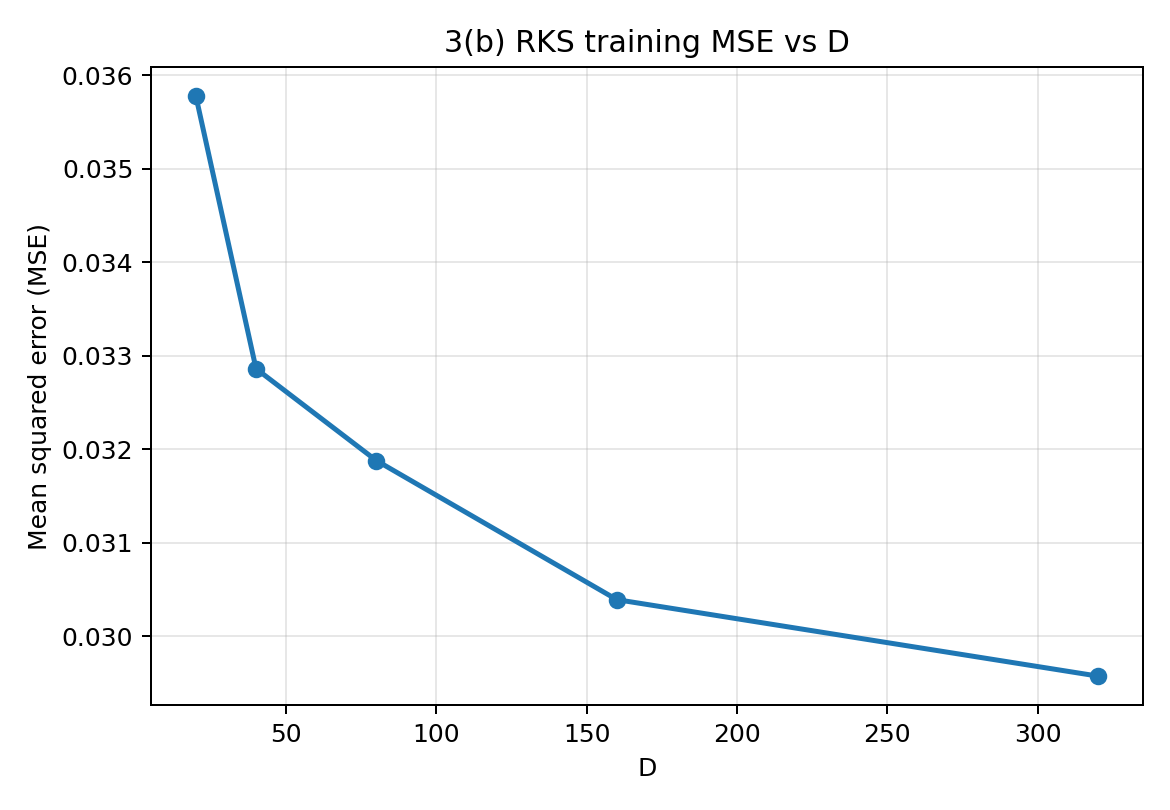
\includegraphics[width=\linewidth]{figures/3b_rks_training_mse.png}
\caption*{\textit{Figure 6a. RKS training MSE vs D.}}
\end{minipage}\hfill
\begin{minipage}[t]{0.485\linewidth}
\centering
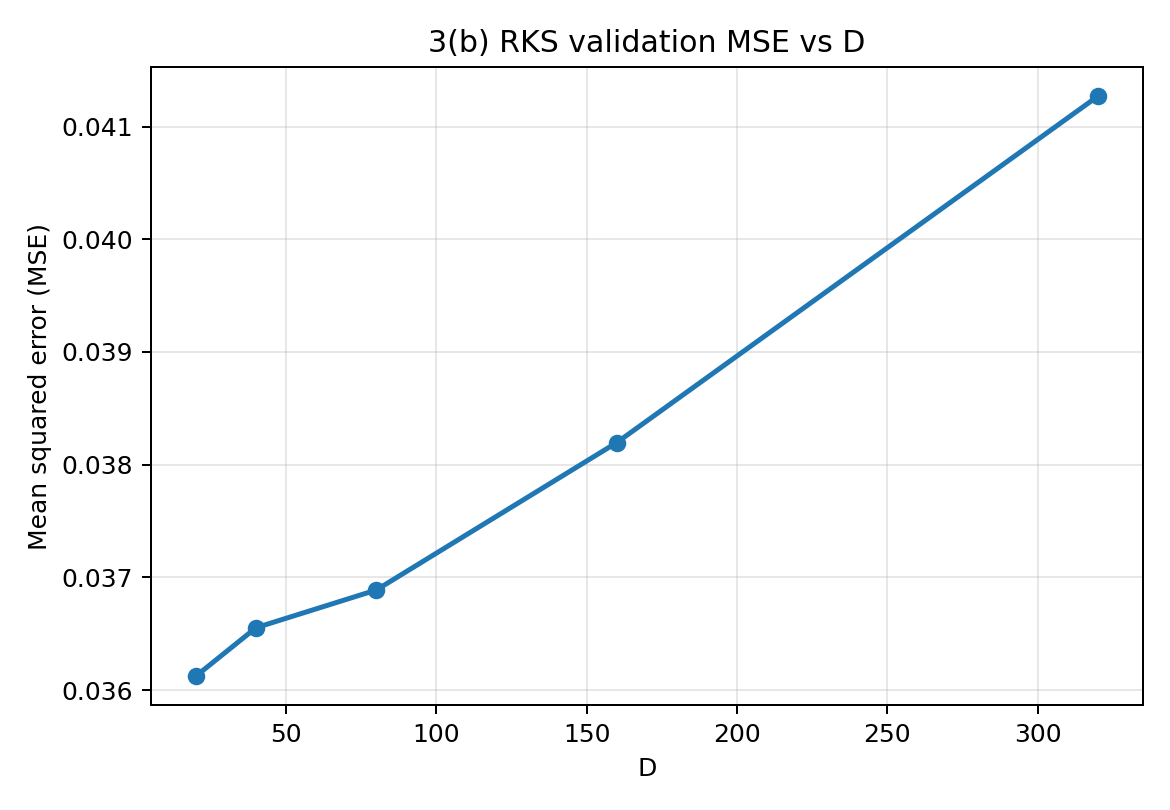
\includegraphics[width=\linewidth]{figures/3b_rks_validation_mse.png}
\caption*{\textit{Figure 6b. RKS validation MSE vs D; selected D = 20.}}
\end{minipage}
\end{figure}


\subsection{3(c) One-hidden-layer MLP}\label{c-one-hidden-layer-mlp}

We trained an MLP with input dimension 2, one ReLU hidden layer, and a
linear scalar output. The hidden representation is learned by
backpropagation rather than fixed at random. Keeping Adam learning rate
0.002, batch size 64, and early-stopping patience 45 fixed, we swept
hidden widths \{16, 32, 64, 128\} with up to 600 epochs per candidate.

\begin{center}
\begingroup
\small
\setlength{\tabcolsep}{4pt}
\renewcommand{\arraystretch}{1.18}
\rowcolors{2}{pale}{white}
\begin{tabular}{>{\raggedright\arraybackslash}p{0.220\linewidth}>{\raggedright\arraybackslash}p{0.176\linewidth}>{\raggedright\arraybackslash}p{0.238\linewidth}>{\raggedright\arraybackslash}p{0.246\linewidth}}
\rowcolor{navy}
\textcolor{white}{\textbf{Hidden width}} & \textcolor{white}{\textbf{Best epoch}} & \textcolor{white}{\textbf{Train MSE}} & \textcolor{white}{\textbf{Validation MSE}} \\
16 & 524 & 0.037643 & 0.042134 \\
32 & 279 & 0.036007 & 0.042949 \\
64 & 407 & 0.030971 & 0.039303 \\
128 & 204 & 0.031993 & 0.038674 \\
\end{tabular}
\endgroup
\end{center}

The lowest validation MSE occurs at 128 hidden units (0.038674). A wider
model can represent more detail; the validation curves, rather than
training fit alone, determine selection.

\begin{figure}[H]
\centering
\begin{minipage}[t]{0.485\linewidth}
\centering
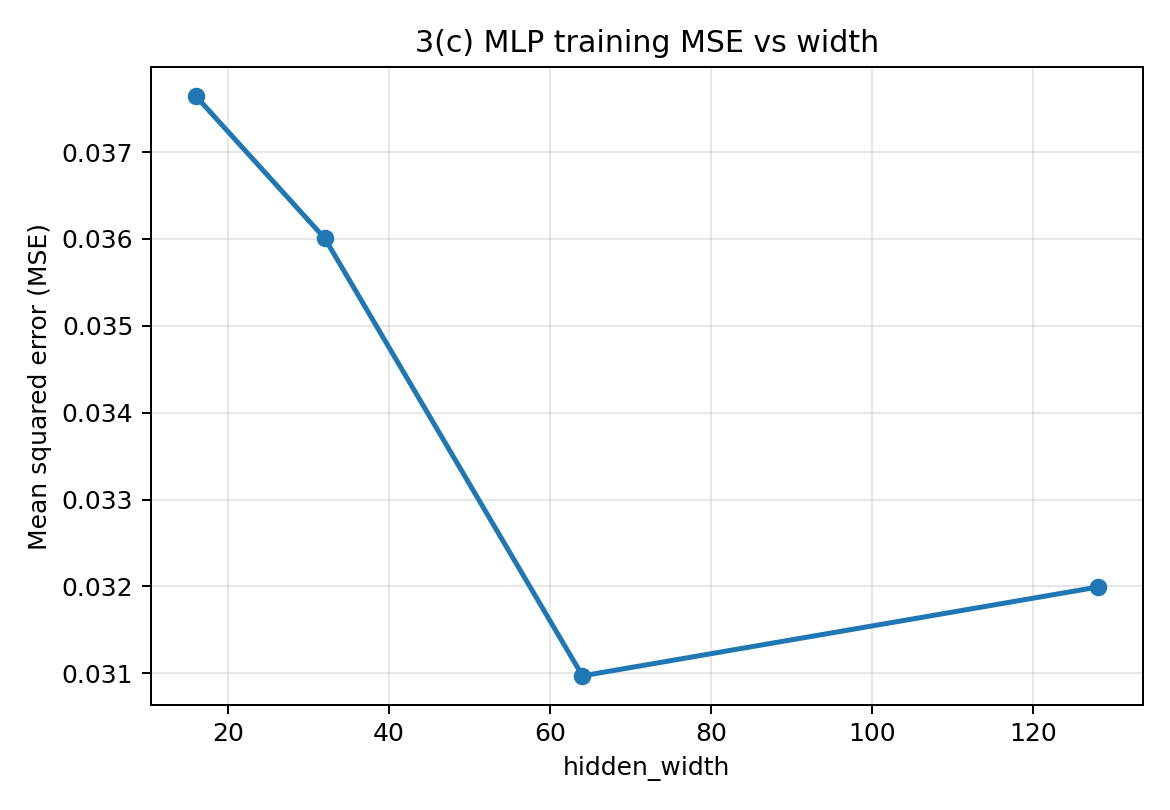
\includegraphics[width=\linewidth]{figures/3c_mlp_training_mse.png}
\caption*{\textit{Figure 7a. MLP training MSE vs hidden width.}}
\end{minipage}\hfill
\begin{minipage}[t]{0.485\linewidth}
\centering
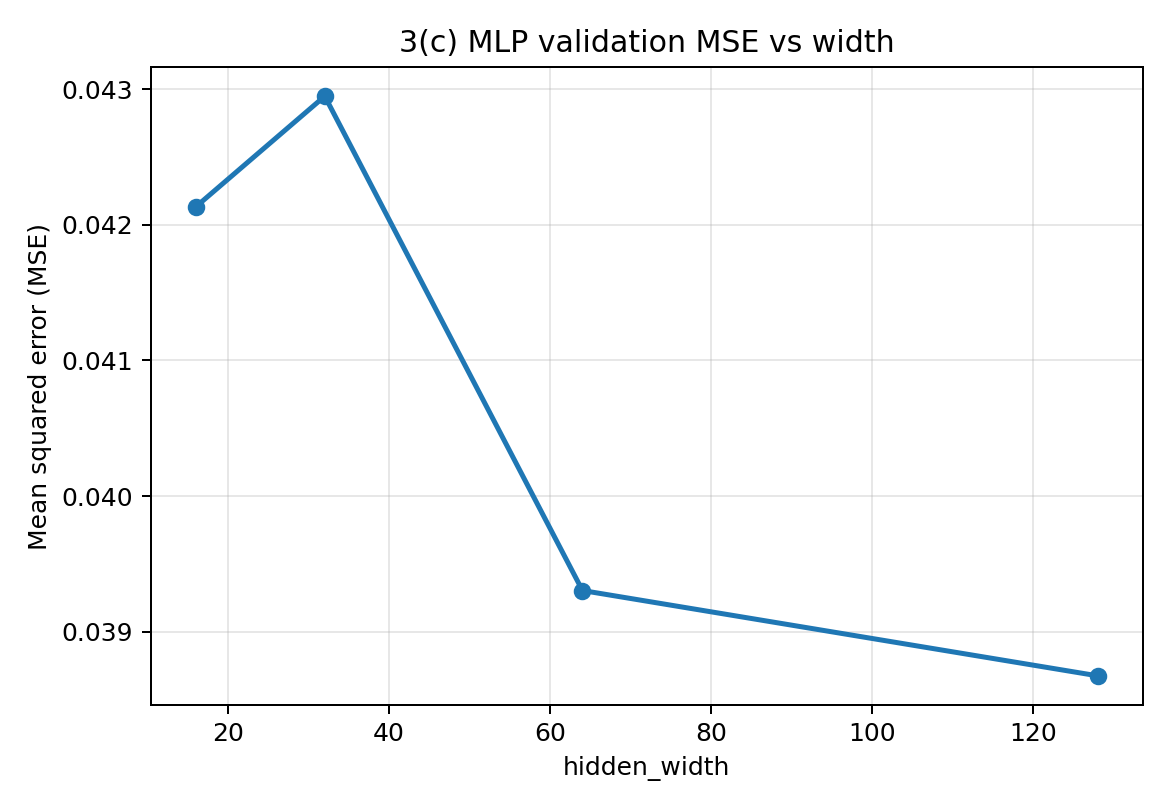
\includegraphics[width=\linewidth]{figures/3c_mlp_validation_mse.png}
\caption*{\textit{Figure 7b. MLP validation MSE vs hidden width.}}
\end{minipage}
\end{figure}

\subsection{3(d) Refit, compare, export test predictions, and visualize
fitted
surfaces}\label{d-refit-compare-export-test-predictions-and-visualize-fitted-surfaces}

Using the validation-selected settings, both models were refit on the
original training split. The held-out validation MSEs are 0.036124 for
RKS (D=20) and 0.038674 for MLP (hidden width 128); RKS performs
slightly better on this split. We generated predictions for the 200-row
unlabeled test set, preserving its order, and exported headerless,
one-column files \path{rks_test_predictions.csv} and
\path{mlp_test_predictions.csv}. No test MSE is reported because test.csv
contains no target column.

\begin{center}
\begingroup
\small
\setlength{\tabcolsep}{4pt}
\renewcommand{\arraystretch}{1.18}
\rowcolors{2}{pale}{white}
\begin{tabular}{>{\raggedright\arraybackslash}p{0.141\linewidth}>{\raggedright\arraybackslash}p{0.343\linewidth}>{\raggedright\arraybackslash}p{0.194\linewidth}>{\raggedright\arraybackslash}p{0.202\linewidth}}
\rowcolor{navy}
\textcolor{white}{\textbf{Model}} & \textcolor{white}{\textbf{Selected configuration}} & \textcolor{white}{\textbf{Train MSE}} & \textcolor{white}{\textbf{Validation MSE}} \\
RKS & D=20 & 0.035776 & 0.036124 \\
MLP & hidden\_width=128 & 0.031993 & 0.038674 \\
\end{tabular}
\endgroup
\end{center}

\begin{center}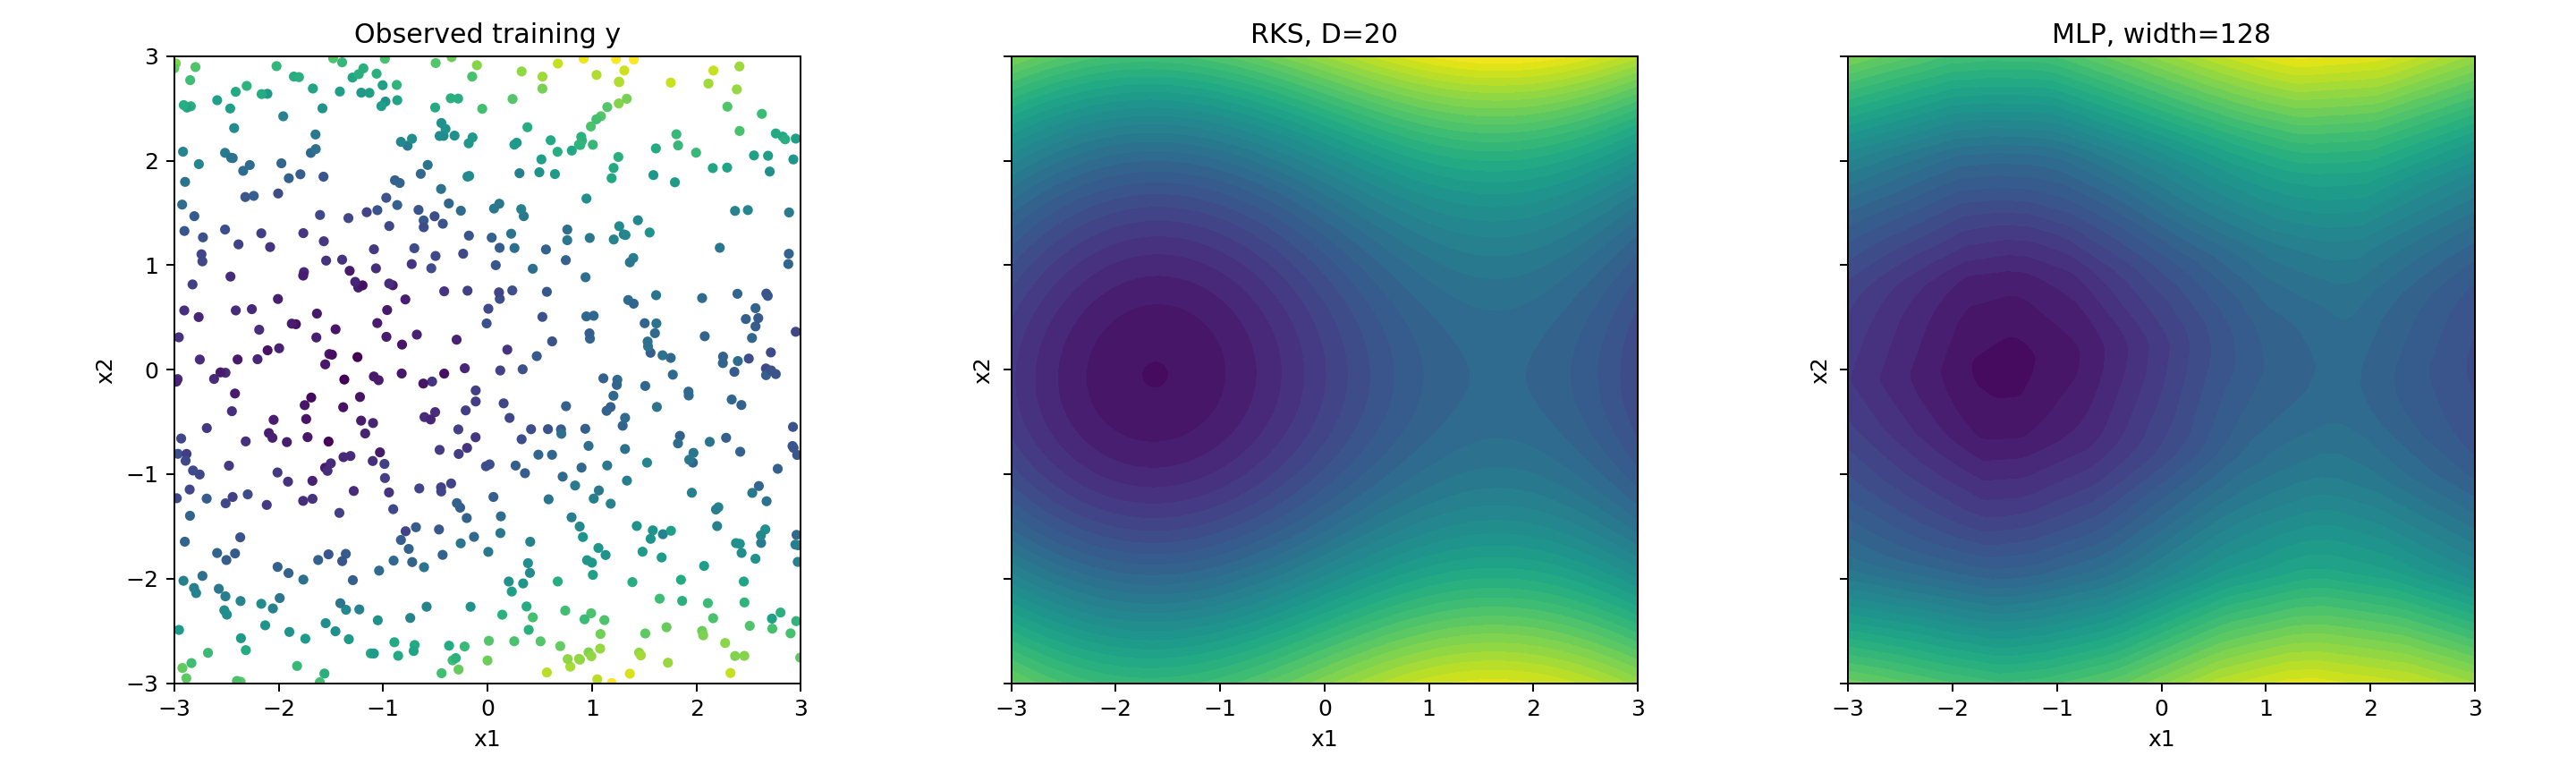
\includegraphics[width=0.96\linewidth]{figures/3d_three_panel_comparison.png}\end{center}

{\footnotesize\itshape\color{muted} Figure 8. Observed training values and both fitted response surfaces, shown on the common input region {[}−3,3{]}².}

Both models capture the broad trough near the left-center and larger
values near the upper and lower boundaries. RKS produces a smooth
sinusoidal approximation; the ReLU MLP creates a slightly more
angular/piecewise-linear surface, which is natural for a network with
ReLU activations. Despite lower MLP training error (0.031993 vs
0.035776), the RKS validation error is lower, an instructive example of
why model selection should use validation rather than training fit. The
next subsection checks how robust both selections are and why RKS comes
out ahead.

\subsection{Robustness of the selections in 3(b)--(c), and why RKS does better in 3(d)}\label{robustness}

Both selected values lie at the end of their grids (D=20 is the
smallest D tried, 128 the largest width), so we checked wider grids and
repeated every setting with other random seeds
(\texttt{code/problem3\_robustness.py}, Figure 9). The selection rule and
the submitted predictions are unchanged.

\textbf{RKS.} Below D=20 the validation MSE rises sharply (0.089 at D=18,
0.137 at D=16), so the optimum is not hidden below the grid. D=24 and 30
are marginally lower with the same seed (0.0349 and 0.0351). However,
with only ten random frequencies the result depends strongly on which
frequencies are drawn: over 20 other draws, D=20 averages 0.140 (standard
deviation 0.137). From D=40 upward the draw no longer matters (0.0380 ±
0.0013 at D=40). The submitted seed happens to draw frequencies that suit
this surface; D≈40--80 is the safer choice when the draw is not fixed. The
mild overfitting at large D comes from the weak penalty: at D=320,
raising λ from 0.01 to 1--10 brings validation MSE from 0.0413 back to
about 0.0383.

\textbf{MLP.} Widths 256, 512 and 1024, each trained with five
initialization seeds (seed 42 and four others), give no improvement beyond
seed-to-seed noise: the five-seed validation means are 0.0383 (128),
0.0381 (256), 0.0384 (512) and 0.0382 (1024), while the seed-to-seed
standard deviation is about 0.0005. Width 128 therefore sits on a plateau,
not at the edge of a decreasing curve.

\textbf{Why D=20 and width 128 are kept.} The grids in 3(b) and 3(c) were
fixed before looking at results, and the wider grids are a diagnostic, not
a second round of selection. Re-selecting D=24 because it is 0.0012 lower
with one random draw would tune to that draw: the difference is a tenth of
the draw-to-draw spread at D=20--24 and a third of the standard error of a
200-point validation MSE (0.0035).

\begin{center}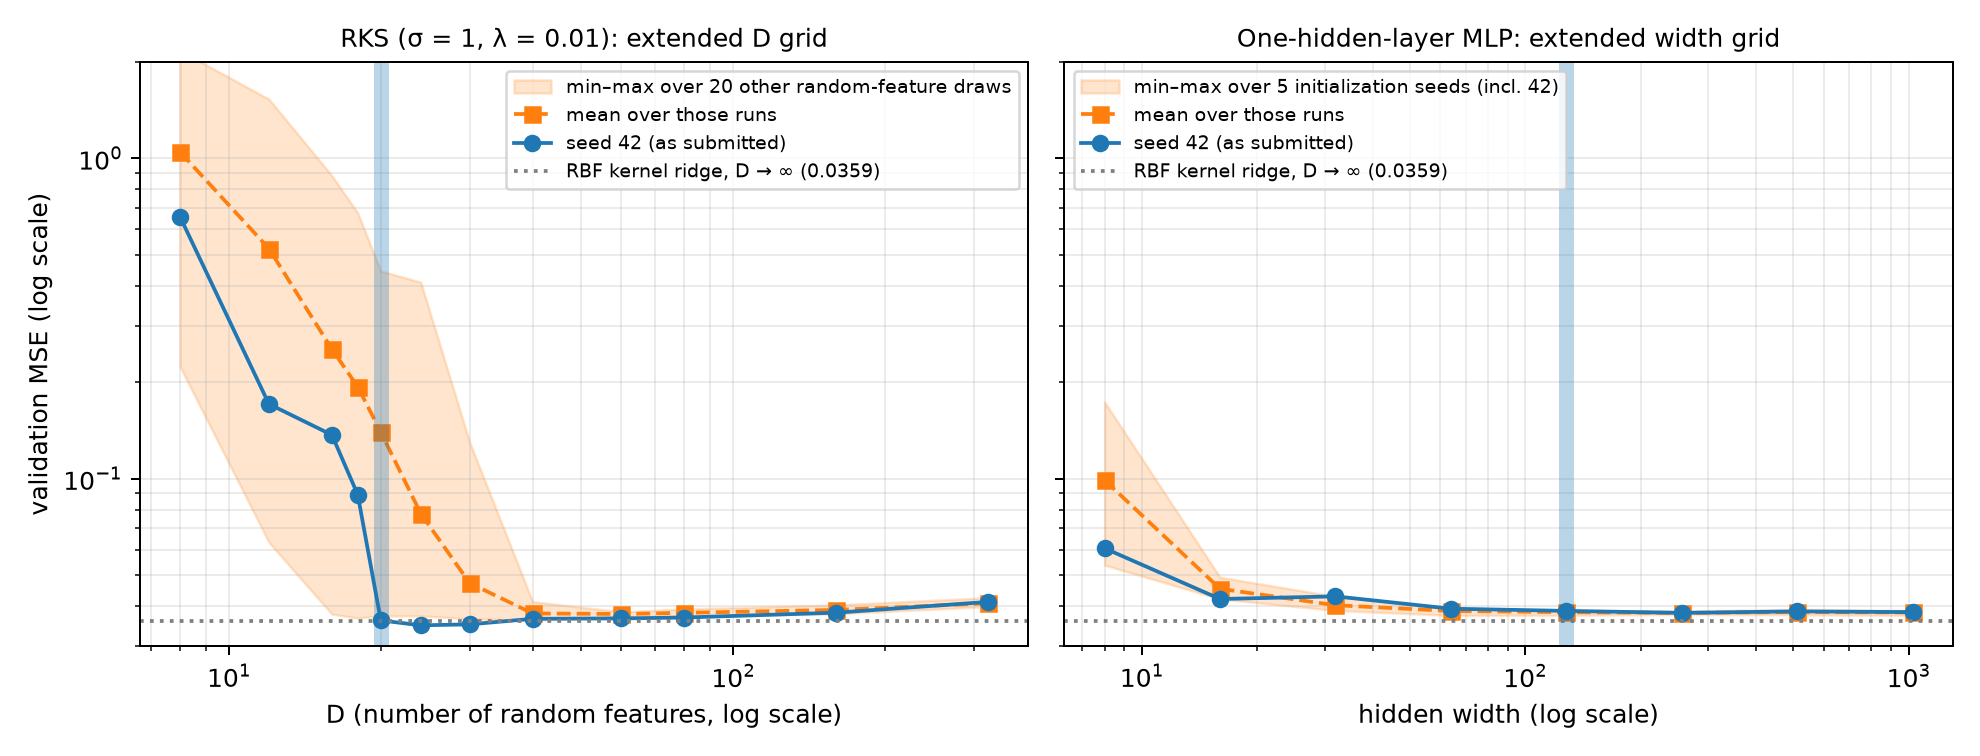
\includegraphics[width=0.98\linewidth]{figures/3e_robustness.png}\end{center}

{\footnotesize\itshape\color{muted} Figure 9. Wider grids with repeated random seeds. Blue: the submitted seed; orange: mean and min--max range over 20 other random-feature draws (RKS) or 5 initialization seeds (MLP); dotted: best RBF kernel ridge fit. Vertical bars mark the submitted choices. Log scales.}

\textbf{Why RKS does slightly better, and how much that means.} First,
both models are already close to the best a smooth regression achieves
on this data. The variance of y is 2.46, so both explain about 98.5\% of
it. As D→∞, RKS ridge becomes RBF kernel ridge; tuning that kernel's
width and penalty on validation gives 0.0359 (at lengthscale 4, i.e. a
smoother kernel than the σ=1 used in 3(b)), essentially the RKS value of
0.0361. Second,
the gap is not statistically resolved: on the same 200 validation points
the MLP-minus-RKS squared error is 0.0026 ± 0.0021 (paired standard
error), and a single 200-point validation MSE has a standard error of
about 0.0035. Third, the direction of the gap has a structural
explanation. The pattern in Figure 5 varies smoothly across the input
square, and Gaussian random
Fourier features encode exactly that smoothness assumption; ridge then
solves a convex problem exactly. The ReLU MLP has to learn its basis by
stochastic optimization and builds a smooth surface from piecewise-linear
pieces, so it fits the training points more closely without generalizing
better. Finally, part of the RKS advantage at D=20 is the particular
random draw: averaged over draws and seeds, RKS at D=40 (0.0380) and the
MLP at width 128 (0.0383) are tied within their spread.

\section{Reproducibility notes and evaluation
integrity}\label{reproducibility-notes-and-evaluation-integrity}

Code and data are in \path{homework_2/} of the course repository
(scripts in \path{code/}, generated outputs in \path{outputs/}):

\hspace*{1.2em}\texttt{pip install -r requirements.txt}\\
\hspace*{1.2em}\texttt{python run\_all.py -{}-smoke}\hfill{\small(input and package checks only)}\hspace*{1.2em}\\
\hspace*{1.2em}\texttt{python run\_all.py -{}-problem 1}\hfill{\small(or 2, 3, robustness, figures, all)}\hspace*{1.2em}

Problem 1 (\path{code/problem1_taxi.py}): the rerun reproduces the
table in 1(e) exactly. The Gaussian curves in Figure 1 are illustrative.

Problem 2 (\path{code/problem2_retail.py}): the baseline and ridge
metrics reproduce exactly; the two neural models agree to about three
decimal places across PyTorch versions, with the same ranking. The
row-level test set is used only for final reporting.

Problem 3 (\path{code/problem3_rks_mlp.py}): the submitted
\path{rks_test_predictions.csv} and \path{mlp_test_predictions.csv}
(in \path{submissions/}) each have 200 finite values in the row order
of test.csv. The robustness check (\path{code/problem3_robustness.py},
about 3 minutes) produces Figure 9 and the numbers in the robustness
subsection; it does not use test.csv.

For all three problems, data, split, target transformation, loss, model
selection criterion, and final evaluation must be distinguished.
Test-dependent model tuning would invalidate the meaning of a held-out
test score.

\end{document}
